%% DO NOT MOVE/EDIT THE FOLLOWING THREE LINES! (used by make.sh)
%\documentclass[notes=only]{beamer}
\documentclass{beamer}
%\setbeameroption{show notes}
%% now you can change again ;)

%% DOCUMENTATION
% http://www2.informatik.hu-berlin.de/~mischulz/beamer.html
% ftp://ftp.mpi-sb.mpg.de/pub/tex/mirror/ftp.dante.de/pub/tex/macros/latex/contrib/beamer/doc/beameruserguide.pdf
% ftp://dante.ctan.org/tex-archive/help/Catalogue/entries/prosper.html
% http://en.wikibooks.org/wiki/LaTeX/Presentations

% HINTS
% http://www.disk0s1.de/posts/latex/beamer-und-fill/

%% HEADERS TODO ???
\usepackage[ngerman]{babel}
\usepackage[utf8x]{inputenc}
\usepackage{amsmath,amsfonts,amssymb,multirow,hyperref}
% http://en.wikibooks.org/wiki/LaTeX/Tables
\usepackage{array} % table

% notes
% http://www.physik.uni-freiburg.de/~tooleh/latex_beamerkurs.pdf
% http://mo.mathematik.uni-stuttgart.de/inhalt/aussage/aussage1326/
%\usepackage{pgfshade}

% http://deic.uab.es/~iblanes/beamer_gallery/index.html
\usetheme{Frankfurt}
\usecolortheme{rose}
\beamertemplatenavigationsymbolsempty
\setbeamertemplate{footline}[frame number]
\setbeamercovered{transparent}
\useoutertheme[subsection=false]{smoothbars}
\useinnertheme{rectangles}

% colors % TODO: better!
\definecolor{vebu-up}{HTML}{E5CF83} % VEBU: sand
\definecolor{vebu-middle}{HTML}{67B821} % VEBU: basis grasgruen
\definecolor{vebu-low}{HTML}{B3DB10} % VEBU: lindgruen
\setbeamercolor{titlelike}{fg=black, bg=vebu-low}
\setbeamercolor{frametitle}{fg=black, bg=vebu-low}
%\setbeamercolor{section in head/foot}{fg=black, bg=vebu-up}
\setbeamercolor{subsection in head/foot}{fg=black, bg=vebu-middle}

% Stuff for the titlepage
\title[YAVA]{YAVA: Yet Another Vegan App}
\subtitle{Abschlusspräsentation}
\author[Y. Haupenthal]{Yannic Haupenthal}
\institute[UdS]{Universität des Saarlandes}
\date[05.08.2013]{05. August 2013}
\subject{YAVA}
\keywords{vegan, app, yava}

% Fix: Numbers instead of letters (footnote)
% http://tex.stackexchange.com/questions/68887/how-do-i-change-footnote-in-beamer
\renewcommand\thempfootnote{\arabic{mpfootnote}}

% dual screen presi mode
% TODO: dual screen: http://www.tug.org/pracjourn/2010-1/dohmen/dohmen.pdf
% http://www.uninformativ.de/projects/?q=slinp


%% ACTUAL PRESENTATION
\begin{document}

% Title
\frame{
	\titlepage
}

% Fundamentals
\begin{frame}{Grundlagen}
		\begin{block}{(Ovo-Lacto-)Vegetarismus}
		- Ernährungsweise\\
		- schließt Verzehr von Lebewesen aus\\
		- tierische ``Produkte'' nicht unbedingt (z.\,B. Milch, Ei,
		Honig)
	\end{block}

	\begin{block}{Veganismus}
		- Lebenseinstellung\\
		- schließt Verzehr aller tierischen ``Produkte'' aus\\
		- lehnt Nutzung von Tieren ab
	\end{block}

	\begin{block}{Veganität}
		bezeichnet wie bzw. ob etwas vegan ist
	\end{block}
\end{frame}

% Overview
\frame{
	\frametitle{Übersicht}
	\tableofcontents
}

\section{Motivation}
\subsection*{Probleme}
\begin{frame}{Probleme}
	\begin{itemize}
		\item Namensunklarheit: E-Nummern, chemische
				Bezeichnungen, Colour Index
		\item Fremdsprachen: Englisch, Latein, Französisch
		\item Ausgangsmaterialien: pflanzlichen, tierischen oder
				mikrobiologischen Ursprungs
		\item Herstellungsprozess: Schönung/Klärung von Getränken,
				Gelatine als Trägerstoff für Vitamine
		\item Produktanfragen: notwendig, aber überall verstreut
		\item Daten: keine freie Datenbank mit Zutatenlisten
	\end{itemize}
\end{frame}

\section{Ziel}
\subsection*{}
\begin{frame}{Ziel}
	\vskip0pt plus 1filll
	\begin{exampleblock}{}
		\begin{itemize}
			\item Website und mobile Apps mit Produktdatenbank
			\item Freie Daten
			\item Plattformunabhängig
			\item Nutzer*innenbasiert
			\item Fokus auf Veganismus (automatische Bestimmung)
		\end{itemize}
	\end{exampleblock}
	\vskip0pt plus 1filll
\end{frame}

\begin{frame}{Aufbau}
	\centering
	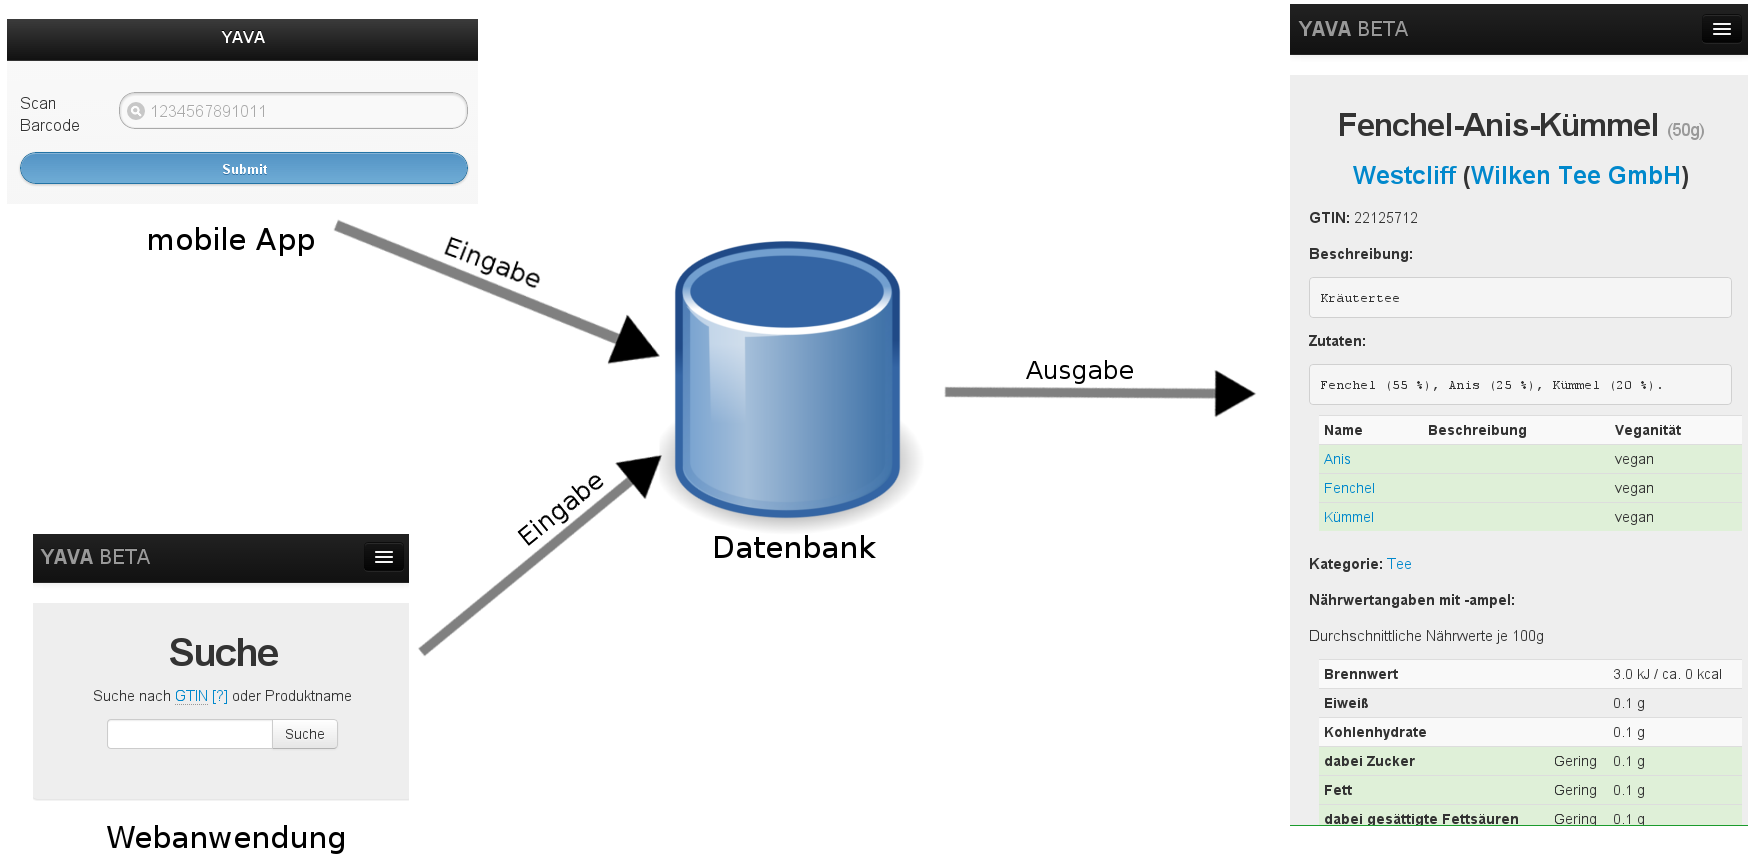
\includegraphics[scale=0.19]{pics/konzept-2.png}
\end{frame}

\section{Verwandte Arbeiten}
\subsection*{related-work}
\begin{frame}{Verwandte Arbeiten}
	\vskip0pt plus 1filll
	\begin{columns}
		\column{.50\textwidth}
			\centering
			%\includegraphics[scale=0.2]{pics/barcoo_logo-500px.png}
		\column{.50\textwidth}
			\centering
			%\includegraphics{pics/das-ist-drin-de_logo_cmyk.jpg}
	\end{columns}

	\begin{columns}
		\column{.50\textwidth}
			\centering
			%\includegraphics[scale=0.1]{pics/eula.png}
		\column{.50\textwidth}
			\centering
			%\includegraphics[scale=0.5]{pics/wikifood-logo.png}
	\end{columns}

	\vskip0pt plus 1filll
	\par\hrulefill\par
	\tiny{Quellen:
    Bretz, A. (2007). \textbf{RFID als Technik für Mobile Health bei
	Lebensmittelallergikern.}}\\
    Arens, A., Rösch, N., Feidert, F., Harpes, P., Herbst, R., \&
    Mösges, R. \textbf{Mobile electronic patient diaries with barcode based
    food identification for the treatment of food allergies.} \textit{GMS Med.
    Inform. Biom. Epidemiol, 4(3).}
\end{frame}

\subsection*{Freiheit}
\begin{frame}{Freiheit der Daten}
	\vskip0pt plus 1filll
		\begin{tabular}{|c|c|c|c|c|}
				\hline
				& Barcoo & d-i-d & EuLa-A & WikiFood\\
				\hline
			Freiheit der Daten & nein & nein & nein & nein\\
				\hline
		\end{tabular}

	\vskip0pt plus 1filll
	\begin{exampleblock}{YAVA}
		\begin{itemize}
			\item Datenbank (PostgreSQL 9)
			\item wichtigste Tabellen: Produkte, Zutaten, Nutzer*innen
			\item Dump kann heruntergeladen werden
		\end{itemize}
	\end{exampleblock}
	
	\vskip0pt plus 1filll
\end{frame}

\subsection*{Plattformübergreifend}
\begin{frame}{Plattformübergreifend}
	\vskip0pt plus 1filll
		\begin{tabular}{|c|c|c|c|c|}
				\hline
				& Barcoo & d-i-d & EuLa-A & WikiFood\\
				\hline
				Plattformübergreifend & ja & ja & nein & ja\\
				\hline
	\end{tabular}
	\vskip0pt plus 1filll


	\begin{exampleblock}{YAVA}
	\begin{itemize}
			\item Website und mobile Apps
			\item Website auf Ruby-on-Rails 4
					mit Bootstrap (Responsive Web Design)
			\item HTML 5, CSS 3, JavaScript
			\item mobile Apps mit PhoneGap 3
	\end{itemize}
	\end{exampleblock}
	\vskip0pt plus 1filll
\end{frame}

\subsection*{Ursprung}
\begin{frame}{Ursprung der Daten}
	\vskip0pt plus 1filll
		\begin{tabular}{|c|c|c|c|c|}
				\hline
				& Barcoo & d-i-d & EuLa-A & WikiFood\\
				\hline
				Nutzer*innenbasiert & nein & ja & nein & (ja)\\
				\hline
	\end{tabular}
	\vskip0pt plus 1filll

	\begin{exampleblock}{YAVA}
	\begin{itemize}
		\item Website mit Login via OAuth2
		\item Anreiz durch Punktbelohnung
		\item fast alle Daten änderbar
	\end{itemize}
	\end{exampleblock}
	\vskip0pt plus 1filll
\end{frame}

\subsection*{Veganität}
\begin{frame}{Veganität (Übersicht)}
	\vskip0pt plus 1filll
	\vskip0pt plus 1filll
		\begin{tabular}{|c|c|c|c|c|}
				\hline
				& Barcoo & d-i-d & EuLa-A & WikiFood\\
				\hline
				Veganität & (ja) & (ja) & nein & (nein)\\
				\hline
	\end{tabular}

	\vskip0pt plus 1filll
	\begin{exampleblock}{}
	\centering
	%\includegraphics[scale=0.2]{pics/veganitaet.png}
	\begin{itemize}
			\item Zutaten: automatische Bestimmung der
					Veganität durch vorhandene Zutaten (Scan durch
					Parser)
			\item Produktanfragen: langsame Veganitätsbestimmung durch
					E-Mail an Hersteller*in (automatisch generiert)
			\item Kommentare: schnelle Sicherstellung der Veganität
				\end{itemize}
		\end{exampleblock}
	\vskip0pt plus 1filll
\end{frame}


\begin{frame}{Veganität (Berechnung)}
	\centering
	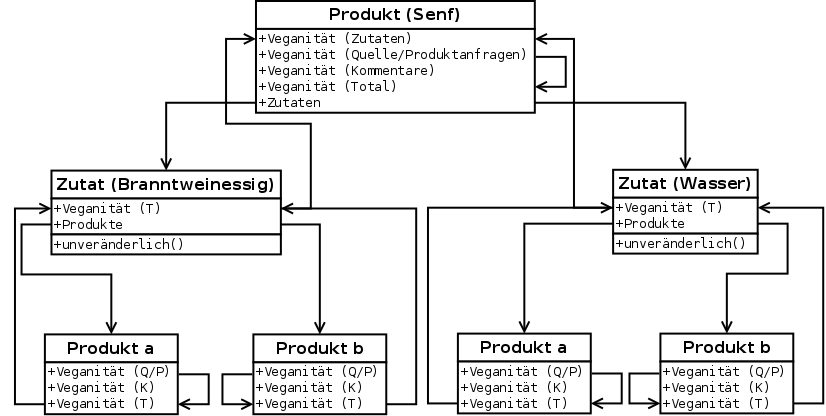
\includegraphics[scale=0.25]{pics/calculate_veganity_de.png}\\
\end{frame}


\section{Ausblick}
\subsection*{Ausblick}
\begin{frame}{Ausblick}
	\vskip0pt plus 1filll
	\begin{itemize}
			\item TODO: Integration im IRL
			\item Parsererweiterung
			\item Veganitätsbestimmung durch Logik
			\item Produktanfragengenerierung verbessern
			\item Einbau von anderen Arbeiten (Orientierungshilfe,
					Augmented Reality, ..)
	\end{itemize}
	\vskip0pt plus 1filll
	\par\hrulefill\par
	\tiny{Quelle:
	Spassova, L., Schöning, J., Kahl, G., \& Krüger, A. (2009).
	\textbf{Innovative retail laboratory.} In \textit{Roots for
	the Future of Ambient
    Intelligence. European Conference on Ambient Intelligence
	(AmI-2009), oA, Salzburg, Austria (November 2009).}}

\end{frame}

\section{Demo}
\subsection*{Demo}
\begin{frame}{Demo}
		\centering
		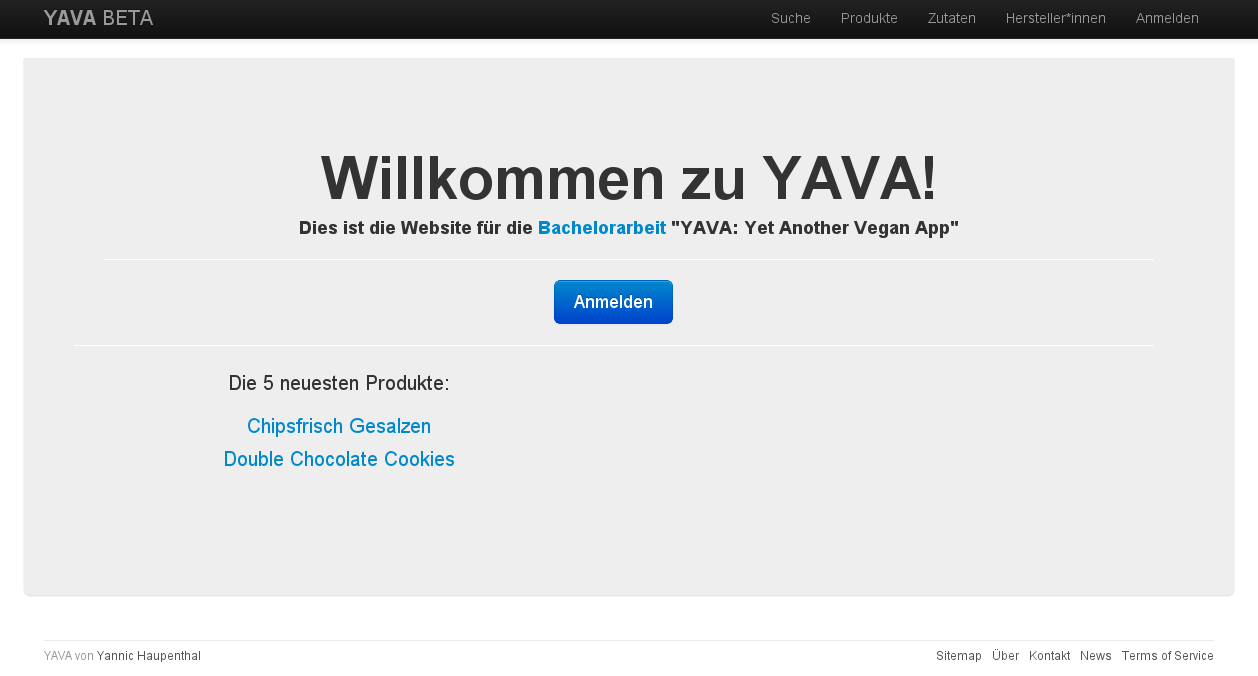
\includegraphics[scale=0.25]{pics/yava-demo.png}
\end{frame}

% don't include the following frames in the header (smoothbars)
% -> define another part
\part{End}

%% End %%

% Thanks
\begin{frame}{Vielen Dank ...}
\begin{center}
	... für die Aufmerksamkeit!
\end{center}
\end{frame}

% Questions
\begin{frame}{Fragen}
\begin{center}
	
\includegraphics[scale=0.2]{pics/qm.png}
\end{center}
\end{frame}

% Backupslide
\begin{frame}{PhoneGap}
	\vskip0pt plus 1filll
	\begin{center}
		%\includegraphics[scale=0.2]{pics/build-diagram-2.png}
	\end{center}
	\vskip0pt plus 1filll
	\begin{itemize}
		\item JS Libraries: jQuery, jQuery Mobile
		\item PG Plugins: BarcodeScanner
	\end{itemize}
	\vskip0pt plus 1filll
\end{frame}

\end{document}
